\documentclass[11pt,a4paper]{article}

% ─── Packages ───────────────────────────────────────────────────────────────
\usepackage[utf8]{inputenc}
\usepackage[T1]{fontenc}
\usepackage{lmodern}
\usepackage[margin=2.5cm]{geometry}
\usepackage{amsmath,amssymb}
\usepackage{booktabs}
\usepackage{graphicx}
\usepackage{xcolor}
\usepackage{hyperref}
\usepackage{pgfplots}
\usepackage{pgfplotstable}
\usepackage{subcaption}
\usepackage{enumitem}
\usepackage{microtype}
\usepackage{float}
\usepackage{fancyhdr}
\usepackage{multirow}

\pgfplotsset{compat=1.18}
\usepgfplotslibrary{groupplots}

\hypersetup{
  colorlinks=true,
  linkcolor=blue!60!black,
  citecolor=green!50!black,
  urlcolor=blue!70!black,
}

% ─── Custom colors ──────────────────────────────────────────────────────────
\definecolor{cvanilla}{HTML}{4C72B0}
\definecolor{ccompile}{HTML}{DD8452}
\definecolor{ctilegym}{HTML}{55A868}
\definecolor{cpacktg}{HTML}{C44E52}
\definecolor{cliger}{HTML}{8172B3}
\definecolor{cfailed}{HTML}{999999}
\definecolor{lightgray}{HTML}{F5F5F5}

% ─── Header/Footer ──────────────────────────────────────────────────────────
\pagestyle{fancy}
\fancyhf{}
\fancyhead[L]{\small SiQ-VL Training Efficiency}
\fancyhead[R]{\small\thepage}
\renewcommand{\headrulewidth}{0.4pt}

% ─── Title ──────────────────────────────────────────────────────────────────
\title{%
  \textbf{A Practitioner's Guide to Single-GPU Training Efficiency\\
  for Vision-Language Models}\\[6pt]
  \large Systematic Optimization from 4.6K to 101K Tokens/Second
}
\author{
  Victor An \\
  \url{https://github.com/duoan/SiQ_VL}
}
\date{May 2026}

% ═══════════════════════════════════════════════════════════════════════════════
\begin{document}
\maketitle

% ─── Abstract ───────────────────────────────────────────────────────────────
\begin{abstract}
% Context
Training vision-language models (VLMs) efficiently on a single GPU is a prerequisite
for both resource-constrained research and as the per-device building block of distributed
training. Yet no systematic guide exists for the full optimization space---from dtype
selection through kernel fusion to data layout strategies---or documents how these
techniques interact across training stages and model scales.

% Content
We present a complete, reproducible optimization recipe for single-GPU VLM training,
developed iteratively on SiQ-VL (SigLIP-2 + Qwen2.5) running on an NVIDIA Blackwell GPU.
Through controlled experiments at two model scales (0.5B and 1.5B parameters), we identify
five optimization layers---precision, batching, kernel fusion, attention backends, and data
packing---and characterize their interactions. The recipe achieves \textbf{6.86$\times$}
Stage~1 speedup (14.7K$\to$100.9K tokens/s) and \textbf{2.95$\times$} Stage~2 speedup
(29.2K$\to$86.1K tokens/s) on the 0.5B model, and \textbf{6.73$\times$} Stage~1 speedup
on the 1.5B model.

% Conclusion
Our key finding is that optimal configuration is \emph{stage-dependent} and
\emph{scale-dependent}: techniques that accelerate Stage~1 (frozen backbone) can
catastrophically degrade Stage~2 (full fine-tuning), and kernel compatibility varies
across model architectures. We release the full benchmark suite, all experiment traces,
and a decision tree that practitioners can apply to any VLM following the
projector-alignment + instruction-tuning paradigm.
\end{abstract}

\vspace{0.5em}
\noindent\textbf{Keywords:} Vision-Language Models, Training Efficiency, GPU Optimization,
Kernel Fusion, Sequence Packing, Reproducible Benchmarking\\[3pt]
\noindent\textbf{Code \& Data:} \url{https://github.com/duoan/SiQ_VL}

\tableofcontents
\newpage

% ═══════════════════════════════════════════════════════════════════════════════
\section{Introduction}
\label{sec:intro}

% Context (Rule 1: central contribution; Rule 5: tell it like a story)
The two-stage training recipe for vision-language models---projector alignment followed by
instruction tuning---has become the dominant paradigm~\cite{liu2023llava,liu2024llava15}.
While significant engineering effort has gone into \emph{distributed} training
systems~\cite{shoeybi2019megatron,rasley2020deepspeed}, the \emph{single-GPU efficiency
frontier} is equally important: it determines the baseline throughput that data parallelism
multiplies, and it is the only option for researchers on limited hardware.

% Gap
Despite the proliferation of kernel libraries (Liger-Kernel~\cite{hsu2024liger},
Unsloth~\cite{unsloth2024}), attention backends (FlashAttention~\cite{dao2022flashattention,dao2023flashattention2},
FlexAttention~\cite{he2024flexattention}), and data strategies (packing~\cite{krell2021efficient},
bucketing), no systematic study documents:
\begin{enumerate}[leftmargin=*,nosep]
  \item How these techniques compose and interact on modern hardware (Blackwell);
  \item Why the \emph{same kernel} can help in one training stage and hurt in another;
  \item What the practical VRAM--speed Pareto frontier looks like across configurations.
\end{enumerate}

% Contribution (Rule 1: single central contribution)
\paragraph{Central Contribution.}
We provide a \textbf{systematic optimization guide} for single-GPU VLM training that:
\begin{itemize}[leftmargin=*,nosep]
  \item Identifies five optimization layers and their cross-layer interactions;
  \item Validates across two model scales (0.5B and 1.5B) and two training stages;
  \item Documents both successes and failures with root-cause analysis;
  \item Produces a decision tree that practitioners can apply directly.
\end{itemize}

The guide is validated on SiQ-VL but designed to generalize to any VLM following the
projector-alignment paradigm (LLaVA, InternVL, Qwen-VL, PaliGemma, etc.).

% ═══════════════════════════════════════════════════════════════════════════════
\section{Background and Related Work}
\label{sec:related}

\paragraph{VLM Training Paradigm.}
Modern VLMs~\cite{liu2023llava,chen2024internvl,bai2023qwenvl,wang2024qwen2vl} share a
common structure: a frozen vision encoder, a lightweight projector, and a language model
backbone. Training proceeds in stages: Stage~1 aligns visual features to the LLM embedding
space (only projector trains); Stage~2 instruction-tunes the full model or applies
LoRA~\cite{hu2022lora}. This staging creates \emph{fundamentally different} compute
profiles that require different optimization strategies---a key insight of this work.

\paragraph{Kernel Optimization Landscape.}
FlashAttention~\cite{dao2022flashattention,dao2023flashattention2} reduces attention memory
from $O(N^2)$ to $O(N)$. Triton~\cite{tillet2019triton} enables Python-based custom kernels,
powering Liger-Kernel~\cite{hsu2024liger} (fused RMSNorm, SwiGLU, RoPE, cross-entropy for
LLM training). NVIDIA's cuTile DSL (CUTLASS~4.0) provides direct Blackwell hardware access
via TileGym. PyTorch's \texttt{torch.compile}~\cite{ansel2024pytorch} offers zero-dependency
kernel fusion via Inductor. We systematically compare all four approaches.

\paragraph{Data Efficiency.}
Sequence packing~\cite{krell2021efficient} eliminates padding by concatenating samples into
fixed-length bins. Variable-length attention via \texttt{cu\_seqlens} or
FlexAttention~\cite{he2024flexattention} maintains sample isolation. Length
bucketing~\cite{raffel2020t5} groups similar-length sequences to reduce padding without
packing complexity. We quantify when each strategy is worthwhile.

\paragraph{Efficiency Metrics.}
MFU (Model FLOPs Utilization)~\cite{chowdhery2023palm} measures hardware efficiency.
We introduce \textbf{Real tok/s} (non-padding tokens processed per second) as the primary
metric, which captures both hardware throughput and data efficiency in a single number.

% ═══════════════════════════════════════════════════════════════════════════════
\section{The Optimization Framework}
\label{sec:framework}

We organize optimizations into five layers, ordered by implementation effort and
typical impact:

\begin{table}[H]
\centering
\caption{The five-layer optimization framework for VLM training}
\label{tab:framework}
\begin{tabular}{@{}clll@{}}
\toprule
\textbf{Layer} & \textbf{Category} & \textbf{Techniques} & \textbf{Typical Impact} \\
\midrule
1 & Precision & BF16 model loading, mixed precision & 2--3$\times$ \\
2 & Batching & Batch scaling, gradient accumulation & 1.3--1.6$\times$ \\
3 & Data Layout & Length bucketing, sequence packing & 1.1--1.5$\times$ \\
4 & Kernel Fusion & Liger, TileGym, torch.compile & 1.4--2.0$\times$ \\
5 & System Tuning & Grad checkpointing removal, optimizer & 1.1--1.2$\times$ \\
\bottomrule
\end{tabular}
\end{table}

\paragraph{Key Principle: Layers Interact.}
These layers are not independent. Kernel fusion (Layer~4) may require specific input shapes
imposed by data layout (Layer~3). Removing gradient checkpointing (Layer~5) requires VRAM
headroom created by precision (Layer~1) and kernel memory savings (Layer~4). The optimal
configuration is the \emph{composition} that maximizes throughput within the VRAM budget.

% ═══════════════════════════════════════════════════════════════════════════════
\section{Experimental Setup}
\label{sec:setup}

\begin{table}[H]
\centering
\caption{Hardware and model configurations}
\label{tab:setup}
\begin{tabular}{@{}ll@{}}
\toprule
\multicolumn{2}{@{}l}{\textbf{Hardware}} \\
\midrule
GPU & NVIDIA RTX PRO 6000 Blackwell (96\,GB GDDR7) \\
Memory Bandwidth & 1.79\,TB/s \\
Peak BF16 Compute & 936\,TFLOP/s (188 SMs @ 2430\,MHz) \\
CUDA / Driver & CUDA 13.0 / Driver 580.126 \\
\midrule
\multicolumn{2}{@{}l}{\textbf{Small Model (0.5B total)}} \\
\midrule
Vision Encoder & SigLIP2-base-patch16-224 (92.9M, frozen) \\
Language Model & Qwen2.5-0.5B-Instruct (494.0M) \\
Projector & 2-layer MLP + Pixel Shuffle $\times$2 (2.8M) \\
\midrule
\multicolumn{2}{@{}l}{\textbf{Large Model (1.9B total)}} \\
\midrule
Vision Encoder & SigLIP2-so400m-patch14-384 (400M, frozen) \\
Language Model & Qwen2.5-1.5B-Instruct (1.54B) \\
Projector & 2-layer MLP + Pixel Shuffle $\times$3 (9.4M) \\
\midrule
\multicolumn{2}{@{}l}{\textbf{Benchmark Protocol}} \\
\midrule
Dataset & sharegpt4v/coco (50K real VQA samples) \\
Measurement & 20 steps after 5-step warmup, torch.cuda.synchronize \\
Metrics & Real tok/s, VRAM, Pad\%, Speedup vs FP32 baseline \\
\bottomrule
\end{tabular}
\end{table}

\paragraph{Methodology.}
All experiments use a single script (\texttt{benchmark\_real\_efficiency.py}) that runs
actual forward-backward steps on real data---no synthetic benchmarks. Each configuration
runs in an isolated Python subprocess to prevent kernel patch contamination. We measure
wall-clock step time between \texttt{torch.cuda.synchronize()} calls and report
\textbf{Real tok/s} = non-padding tokens / wall time.

% ═══════════════════════════════════════════════════════════════════════════════
\section{Results: Small Model (0.5B)}
\label{sec:results_small}

\subsection{Stage 1: Projector Alignment (Frozen LLM)}

\begin{table}[H]
\centering
\caption{Stage 1 results --- small model (SigLIP2-base-224 + Qwen2.5-0.5B)}
\label{tab:s1_small}
\small
\begin{tabular}{@{}clrrrr@{}}
\toprule
\# & Configuration & Real tok/s & VRAM & Pad\% & Speedup \\
\midrule
1 & Baseline (FP32, B=4) & 14,713 & 10.5\,GB & 12.3\% & 1.00$\times$ \\
2 & BF16 fix, B=4 & 34,747 & 7.1\,GB & 12.3\% & \textbf{2.36$\times$} \\
3 & BF16, B=16 & 45,893 & 25.2\,GB & 16.9\% & 3.12$\times$ \\
4 & BF16, B=16, bucketing & 52,854 & 18.0\,GB & 3.8\% & 3.59$\times$ \\
5 & BF16, B=32, bucketing & 54,136 & 35.1\,GB & 4.4\% & 3.68$\times$ \\
6 & BF16, B=64, bucketing & 51,191 & 69.4\,GB & 5.0\% & 3.48$\times$ \\
\midrule
7 & Liger (+FusedCE), B=32 & 76,252 & 9.5\,GB & 4.4\% & \textbf{5.18$\times$} \\
8 & Liger (no FusedCE), B=32 & 66,029 & 31.7\,GB & 4.4\% & 4.49$\times$ \\
9 & torch.compile, B=32 & 94,342 & 21.9\,GB & 4.4\% & \textbf{6.41$\times$} \\
10 & TileGym, B=32, pad64 & 91,866 & 10.9\,GB & 14.3\% & 6.24$\times$ \\
11 & TileGym, B=64, pad64 & 93,344 & 18.2\,GB & 14.0\% & 6.34$\times$ \\
\midrule
12 & Packing N=1024, B=64 & 57,204 & 72.2\,GB & 0.0\% & 3.89$\times$ \\
13 & \textbf{Packing + TileGym, B=64} & \textbf{100,923} & 18.1\,GB & 0.0\% & \textbf{6.86$\times$} \\
\bottomrule
\end{tabular}
\end{table}

\subsection{Stage 2: Full Fine-tuning (Unfrozen LLM, No Gradient Checkpointing)}

\begin{table}[H]
\centering
\caption{Stage 2 results --- small model. Gradient checkpointing disabled (VRAM budget allows it).}
\label{tab:s2_small}
\small
\begin{tabular}{@{}clrrrr@{}}
\toprule
\# & Configuration & Real tok/s & VRAM & Pad\% & Speedup \\
\midrule
1 & Vanilla, B=4 (baseline) & 29,167 & 7.9\,GB & 12.3\% & 1.00$\times$ \\
2 & Vanilla, B=16, bucketing & 44,934 & 20.3\,GB & 3.8\% & 1.54$\times$ \\
3 & Vanilla, B=32, bucketing & 45,748 & 39.5\,GB & 4.4\% & 1.57$\times$ \\
\midrule
4 & Liger (no FusedCE), B=16 & 52,330 & 18.1\,GB & 3.8\% & 1.79$\times$ \\
5 & Liger (+FusedCE), B=16 & 17,434 & 8.0\,GB & 3.8\% & 0.60$\times$ {\color{red}$\downarrow$} \\
6 & Liger (no FusedCE), B=32 & 55,504 & 35.2\,GB & 4.4\% & 1.90$\times$ \\
\midrule
7 & torch.compile, B=16 & 68,105 & 13.2\,GB & 3.8\% & 2.34$\times$ \\
8 & torch.compile, B=32 & 73,052 & 25.4\,GB & 4.4\% & \textbf{2.50$\times$} \\
\midrule
9 & TileGym, B=16, pad64 & 72,174 & 9.1\,GB & 14.4\% & 2.47$\times$ \\
10 & TileGym, B=32, pad64 & 76,907 & 15.7\,GB & 14.3\% & 2.64$\times$ \\
11 & TileGym, B=64, pad64 & 79,155 & 27.4\,GB & 14.0\% & 2.71$\times$ \\
\midrule
12 & Packing N=1024, B=32 & 51,091 & 44.7\,GB & 0.0\% & 1.75$\times$ \\
13 & \textbf{Packing + TileGym, B=64} & \textbf{86,080} & 27.4\,GB & 0.0\% & \textbf{2.95$\times$} \\
\bottomrule
\end{tabular}
\end{table}

% ═══════════════════════════════════════════════════════════════════════════════
\section{Results: Large Model (1.5B)}
\label{sec:results_large}

\begin{table}[H]
\centering
\caption{Large model results (SigLIP2-so400m-384 + Qwen2.5-1.5B). TileGym incompatible
(head\_dim=72 $\neq$ power of 2).}
\label{tab:large}
\small
\begin{tabular}{@{}clrrrr@{}}
\toprule
\# & Configuration & Real tok/s & VRAM & Pad\% & Speedup \\
\midrule
\multicolumn{6}{@{}l}{\textit{Stage 1 (Frozen LLM)}} \\
\midrule
1 & Baseline (FP32, B=2) & 4,626 & 13.4\,GB & 6.0\% & 1.00$\times$ \\
2 & BF16 fix, B=2 & 13,862 & 7.7\,GB & 6.0\% & \textbf{3.00$\times$} \\
3 & BF16, B=8, bucketing & 20,460 & 16.1\,GB & 2.6\% & 4.42$\times$ \\
4 & BF16, B=16, bucketing & 21,703 & 28.9\,GB & 3.4\% & 4.69$\times$ \\
5 & Liger (no FusedCE), B=16 & 25,532 & 25.0\,GB & 3.4\% & 5.52$\times$ \\
6 & Liger (+FusedCE), B=32 & 26,425 & 22.7\,GB & 4.1\% & 5.71$\times$ \\
7 & \textbf{torch.compile, B=16} & \textbf{31,110} & 19.9\,GB & 3.4\% & \textbf{6.73$\times$} \\
\midrule
\multicolumn{6}{@{}l}{\textit{Stage 2 (Unfrozen LLM, no grad checkpointing)}} \\
\midrule
1 & Vanilla, B=2 (baseline) & 11,569 & 8.5\,GB & 6.0\% & 1.00$\times$ \\
2 & Vanilla, B=16, bucketing & 18,208 & 33.8\,GB & 3.4\% & 1.57$\times$ \\
3 & Liger (no FusedCE), B=16 & 20,899 & 28.9\,GB & 3.4\% & 1.81$\times$ \\
4 & Liger (+FusedCE), B=16 & 10,731 & 18.7\,GB & 3.4\% & 0.93$\times$ {\color{red}$\downarrow$} \\
5 & \textbf{torch.compile, B=16} & \textbf{24,153} & 23.7\,GB & 3.4\% & \textbf{2.09$\times$} \\
\bottomrule
\end{tabular}
\end{table}

% ═══════════════════════════════════════════════════════════════════════════════
\section{Analysis and Insights}
\label{sec:analysis}

\subsection{Cross-Scale Comparison}

\begin{table}[H]
\centering
\caption{Optimization gains are consistent across model scales}
\label{tab:crossscale}
\begin{tabular}{@{}lrrr@{}}
\toprule
Metric & Small (0.5B) & Large (1.5B) & Ratio \\
\midrule
Stage 1 baseline & 14,713 tok/s & 4,626 tok/s & 3.2$\times$ \\
Stage 1 peak & 100,923 tok/s & 31,110 tok/s & 3.2$\times$ \\
Stage 1 speedup & 6.86$\times$ & 6.73$\times$ & $\approx$equal \\
\midrule
Stage 2 baseline & 29,167 tok/s & 11,569 tok/s & 2.5$\times$ \\
Stage 2 peak & 86,080 tok/s & 24,153 tok/s & 3.6$\times$ \\
Stage 2 speedup & 2.95$\times$ & 2.09$\times$ & Large gains less \\
\bottomrule
\end{tabular}
\end{table}

\paragraph{Observation.} Stage~1 speedup is consistent ($\sim$6.7--6.9$\times$) across
scales because the frozen LLM acts as a fixed-cost forward pass where precision and batch
scaling provide proportional benefits. Stage~2 speedup is lower for the large model
(2.09$\times$ vs 2.95$\times$) because the 1.5B model is more compute-bound, leaving
less room for throughput improvement beyond precision and batching.

\subsection{The FusedCE Paradox: Stage-Dependent Kernel Behavior}
\label{sec:fusedce}

The most surprising finding is that Liger-Kernel's \texttt{fused\_linear\_cross\_entropy}
exhibits \textbf{opposite} behavior across stages:

\begin{itemize}[leftmargin=*,nosep]
  \item \textbf{Stage 1} (frozen LLM): FusedCE is beneficial (+15\% throughput, $-$70\% VRAM).
    Only forward runs through the LM head; chunked approach avoids materializing
    $[B {\times} N, V]$ logits.
  \item \textbf{Stage 2} (unfrozen LLM): FusedCE is catastrophic ($-$40 to $-$67\% throughput).
    Backward pass recomputes the chunked forward, issuing many small Triton kernel launches
    that undersaturate Blackwell's 188 SMs.
\end{itemize}

\paragraph{Root Cause.} We isolated this via component-by-component profiling:

\begin{table}[H]
\centering
\caption{Liger component isolation (Stage 2, B=16, grad\_ckpt=ON)}
\label{tab:liger_isolation}
\small
\begin{tabular}{@{}lrrr@{}}
\toprule
Components Enabled & ms/step & VRAM & $\Delta$ vs Vanilla \\
\midrule
Vanilla (none) & 133.6 & 13.4\,GB & --- \\
RoPE only & 132.7 & 13.4\,GB & $-$0.7\% \\
+ RMSNorm & 119.6 & 13.4\,GB & $-$10.4\% \\
+ SwiGLU & 109.0 & 13.4\,GB & $-$18.4\% \\
+ FusedCE (all) & 254.8 & 2.3\,GB & +90.8\% \\
FusedCE only & 284.5 & 2.3\,GB & +113.0\% \\
\bottomrule
\end{tabular}
\end{table}

\paragraph{Takeaway.} Kernel libraries must be configured per-stage. The optimal Liger
configuration is: \texttt{fused\_linear\_cross\_entropy=True} for Stage~1,
\texttt{fused\_linear\_cross\_entropy=False} for Stage~2 on high-VRAM GPUs.

\subsection{Gradient Checkpointing: A Premature Optimization}

Standard practice enables gradient checkpointing for fine-tuning. On a 96\,GB GPU training
a 0.5B model (peak VRAM $<$40\,GB), this is pure overhead:

\begin{table}[H]
\centering
\caption{Gradient checkpointing overhead (Stage 2, 90GB GPU)}
\label{tab:gradckpt}
\begin{tabular}{@{}lrrr@{}}
\toprule
Config & With & Without & Speed Gain \\
\midrule
Vanilla B=16 & 133.4\,ms & 115.3\,ms & +15.7\% \\
Liger (no CE) B=16 & 108.7\,ms & 96.6\,ms & +12.5\% \\
TileGym B=16 & 107.0\,ms & 88.1\,ms & +21.4\% \\
\bottomrule
\end{tabular}
\end{table}

\paragraph{Takeaway.} Only enable gradient checkpointing when peak VRAM exceeds 80\%
of available capacity. On high-VRAM hardware, disabling it is free throughput.

\subsection{TileGym Incompatibility: Architecture Matters}

TileGym's cuTile kernels require power-of-2 tile dimensions. SigLIP2-so400m has
\texttt{head\_dim=72} (1152/16 attention heads), which is incompatible. This means:
\begin{itemize}[leftmargin=*,nosep]
  \item \textbf{Small model} (SigLIP2-base, head\_dim=64): TileGym works, best Pareto.
  \item \textbf{Large model} (SigLIP-so400m, head\_dim=72): TileGym fails,
    \texttt{torch.compile} is the only option.
\end{itemize}

\paragraph{Takeaway.} Always verify kernel compatibility with your specific model's
hidden dimensions \emph{before} committing to a kernel strategy.

\subsection{Batch Scaling Saturation}

Throughput saturates at a model-dependent batch size:
\begin{itemize}[leftmargin=*,nosep]
  \item Small model: saturates at B=16--32 ($\sim$54K tok/s vanilla, $\sim$94K with kernels)
  \item Large model: saturates at B=8--16 ($\sim$21K tok/s vanilla, $\sim$31K with compile)
\end{itemize}
Beyond saturation, larger batches only increase VRAM and step latency without improving
per-second throughput. The saturation point indicates the transition from
\emph{latency-bound} (GPU idle between operations) to \emph{compute-bound} (all SMs busy).

% ═══════════════════════════════════════════════════════════════════════════════
\section{Failed Experiments and Negative Results}
\label{sec:failures}

Documenting failures is as valuable as successes. Each entry follows:
\textbf{Hypothesis $\to$ Result $\to$ Root Cause}.

\begin{enumerate}[leftmargin=*]

\item \textbf{Vision Feature Caching} (0\% gain).
  \textit{Hypothesis:} Pre-extracting SigLIP features eliminates redundant vision forward passes.
  \textit{Result:} No measurable speedup.
  \textit{Root Cause:} With frozen vision encoder under \texttt{torch.no\_grad()}, vision
  forward is already fast ($<$5\% of step time); caching adds I/O overhead that offsets savings.

\item \textbf{Custom Triton Flash Attention} (slower than SDPA).
  \textit{Hypothesis:} A hand-written Triton FA kernel optimized for our shapes will beat SDPA.
  \textit{Result:} 2.3$\times$ slower than PyTorch's native SDPA.
  \textit{Root Cause:} SDPA dispatches to vendor-optimized cuDNN kernels; Triton JIT overhead
  and suboptimal shared memory usage make custom kernels uncompetitive without deep hardware expertise.

\item \textbf{FlexAttention Packing with Variable Lengths} (51\% padding waste).
  \textit{Hypothesis:} FlexAttention with \texttt{create\_block\_mask} enables efficient
  variable-length packed training.
  \textit{Result:} Mask creation overhead + FlexAttention compiled kernel was slower overall.
  \textit{Root Cause:} FlexAttention's block-sparse approach isn't efficient for the
  small block sizes in our short sequences.

\item \textbf{TileGym with Variable Shapes} (5$\times$ regression).
  \textit{Hypothesis:} TileGym works with any input shape.
  \textit{Result:} 5$\times$ slower than vanilla when sequence lengths aren't multiples of 64.
  \textit{Root Cause:} cuTile requires \texttt{pad\_to\_multiple\_of=64}; non-aligned shapes
  trigger slow fallback paths or autotuning loops per shape.

\item \textbf{Liger + torch.compile} (CUDA illegal memory access).
  \textit{Hypothesis:} Combining Liger's fused kernels with torch.compile gives both benefits.
  \textit{Result:} Crashes with CUDA memory errors.
  \textit{Root Cause:} Liger monkey-patches module forward methods; torch.compile traces
  through the patched code and generates incompatible CUDA graphs.

\item \textbf{Gradient Checkpointing + FusedCE in Stage 2} (2$\times$ slowdown).
  \textit{Hypothesis:} FusedCE's VRAM savings enable larger batches in Stage 2.
  \textit{Result:} $+$91\% step time despite 83\% VRAM reduction.
  \textit{Root Cause:} Gradient checkpointing recomputes the chunked forward pass, doubling
  the number of small Triton kernel launches (see Section~\ref{sec:fusedce}).

\end{enumerate}

% ═══════════════════════════════════════════════════════════════════════════════
\section{The Practitioner's Decision Tree}
\label{sec:decision}

Based on our experiments, we distill the optimization process into a decision tree:

\begin{enumerate}[leftmargin=*]
\item \textbf{Fix precision first.} Ensure model parameters are loaded in BF16/FP16
  (not FP32). This alone yields 2--3$\times$ and costs zero engineering effort.

\item \textbf{Scale batch size to saturation.} Increase batch size until throughput
  plateaus. Use length bucketing to minimize padding at larger batches.

\item \textbf{Choose your kernel strategy based on hardware:}
  \begin{itemize}[nosep]
    \item If your vision encoder has power-of-2 head dimensions $\to$ \textbf{TileGym}
      (best speed/VRAM Pareto)
    \item If not, or if you want zero dependencies $\to$ \textbf{torch.compile}
      (excellent speed, higher VRAM)
    \item If VRAM-constrained (24--48\,GB GPU) $\to$ \textbf{Liger with FusedCE}
      (massive VRAM savings, some speed cost in Stage~2)
  \end{itemize}

\item \textbf{Configure kernels per-stage:}
  \begin{itemize}[nosep]
    \item Stage 1: Enable FusedCE (forward-only benefit, large VRAM savings)
    \item Stage 2: Disable FusedCE, disable gradient checkpointing if VRAM permits
  \end{itemize}

\item \textbf{Consider packing only if:}
  \begin{itemize}[nosep]
    \item Your dataset has high length variance (multi-task, mixed image/text)
    \item Bucketing alone leaves $>$10\% padding
    \item Your kernels work well with fixed-length inputs (packing provides exactly this)
  \end{itemize}
\end{enumerate}

% ═══════════════════════════════════════════════════════════════════════════════
\section{Visualization}
\label{sec:figures}

\begin{figure}[H]
\centering
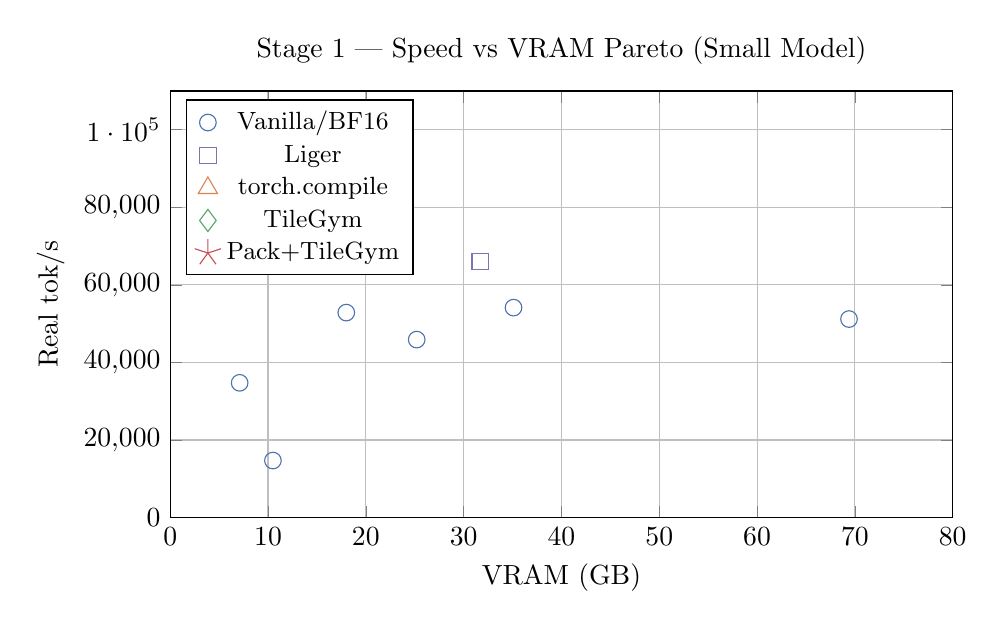
\begin{tikzpicture}
\begin{axis}[
    width=0.95\textwidth, height=7cm,
    xlabel={VRAM (GB)},
    ylabel={Real tok/s},
    xmin=0, xmax=80,
    ymin=0, ymax=110000,
    grid=major,
    legend style={at={(0.02,0.98)}, anchor=north west, font=\small},
    title={Stage 1 --- Speed vs VRAM Pareto (Small Model)},
    scaled y ticks=false,
    yticklabel={\pgfmathprintnumber{\tick}},
]
% Vanilla points
\addplot[only marks, mark=o, color=cvanilla, mark size=3pt] coordinates {
    (10.5, 14713) (7.1, 34747) (25.2, 45893) (18.0, 52854) (35.1, 54136) (69.4, 51191)
};
% Liger
\addplot[only marks, mark=square, color=cliger, mark size=3pt] coordinates {
    (9.5, 76252) (31.7, 66029)
};
% torch.compile
\addplot[only marks, mark=triangle, color=ccompile, mark size=4pt] coordinates {
    (21.9, 94342)
};
% TileGym
\addplot[only marks, mark=diamond, color=ctilegym, mark size=4pt] coordinates {
    (10.9, 91866) (18.2, 93344)
};
% Packing + TileGym
\addplot[only marks, mark=star, color=cpacktg, mark size=5pt] coordinates {
    (18.1, 100923)
};
\legend{Vanilla/BF16, Liger, torch.compile, TileGym, Pack+TileGym}
\end{axis}
\end{tikzpicture}
\caption{Speed--VRAM Pareto frontier for Stage 1. TileGym and Packing+TileGym dominate
the upper-left (high throughput, low VRAM). torch.compile achieves similar speed but at
2$\times$ the VRAM cost.}
\label{fig:pareto_s1}
\end{figure}

\begin{figure}[H]
\centering
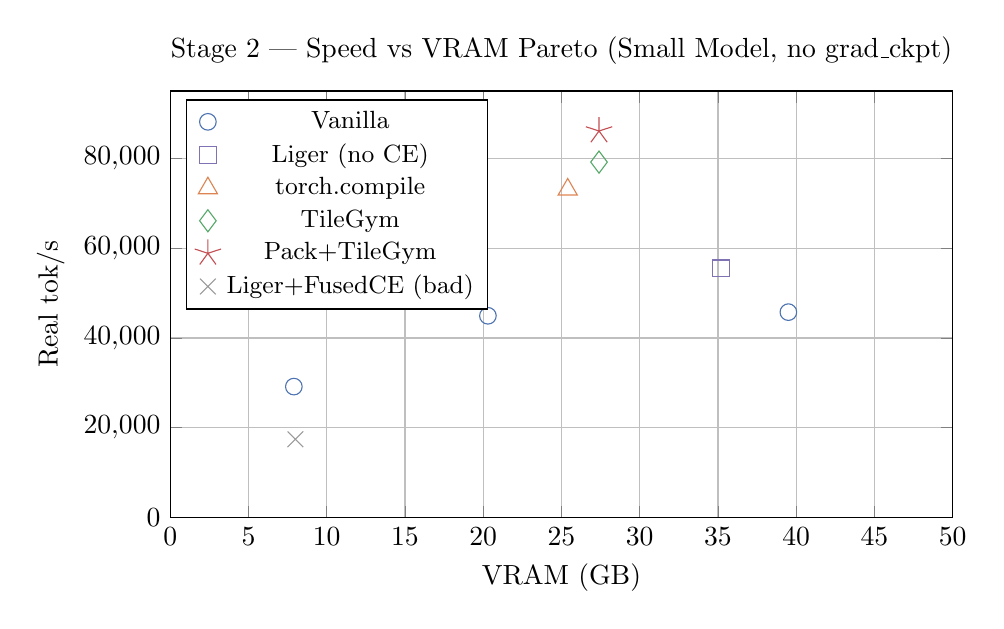
\begin{tikzpicture}
\begin{axis}[
    width=0.95\textwidth, height=7cm,
    xlabel={VRAM (GB)},
    ylabel={Real tok/s},
    xmin=0, xmax=50,
    ymin=0, ymax=95000,
    grid=major,
    legend style={at={(0.02,0.98)}, anchor=north west, font=\small},
    title={Stage 2 --- Speed vs VRAM Pareto (Small Model, no grad\_ckpt)},
    scaled y ticks=false,
    yticklabel={\pgfmathprintnumber{\tick}},
]
% Vanilla
\addplot[only marks, mark=o, color=cvanilla, mark size=3pt] coordinates {
    (7.9, 29167) (20.3, 44934) (39.5, 45748)
};
% Liger (no CE)
\addplot[only marks, mark=square, color=cliger, mark size=3pt] coordinates {
    (18.1, 52330) (35.2, 55504)
};
% torch.compile
\addplot[only marks, mark=triangle, color=ccompile, mark size=4pt] coordinates {
    (13.2, 68105) (25.4, 73052)
};
% TileGym
\addplot[only marks, mark=diamond, color=ctilegym, mark size=4pt] coordinates {
    (9.1, 72174) (15.7, 76907) (27.4, 79155)
};
% Packing + TileGym
\addplot[only marks, mark=star, color=cpacktg, mark size=5pt] coordinates {
    (27.4, 86080)
};
% Failed: Liger with CE
\addplot[only marks, mark=x, color=cfailed, mark size=4pt] coordinates {
    (8.0, 17434)
};
\legend{Vanilla, Liger (no CE), torch.compile, TileGym, Pack+TileGym, Liger+FusedCE (bad)}
\end{axis}
\end{tikzpicture}
\caption{Stage 2 Pareto frontier. TileGym dominates again, but torch.compile is a close
second without external dependencies. Liger with FusedCE ($\times$ marker) is clearly
below the frontier---a cautionary example of blind kernel application.}
\label{fig:pareto_s2}
\end{figure}

\begin{figure}[H]
\centering
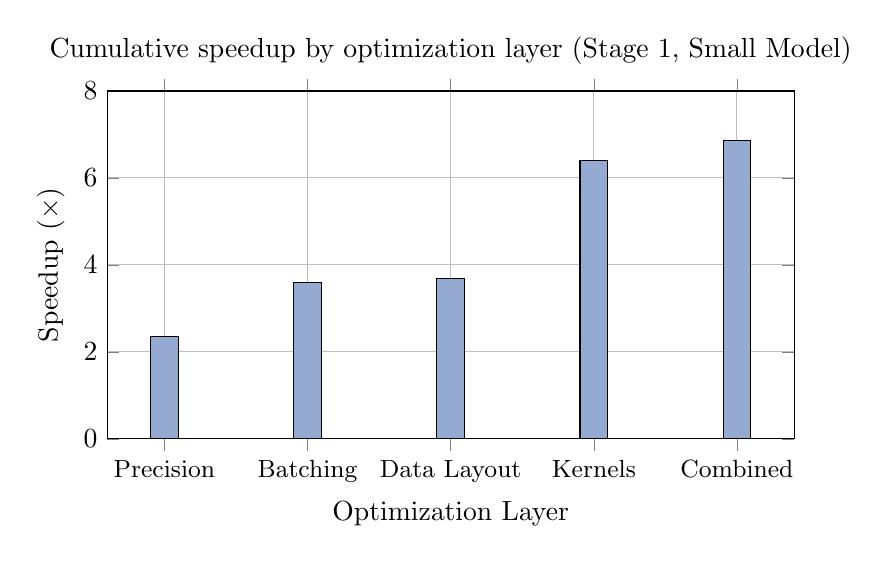
\begin{tikzpicture}
\begin{axis}[
    width=0.85\textwidth, height=6cm,
    ybar,
    bar width=10pt,
    xlabel={Optimization Layer},
    ylabel={Speedup ($\times$)},
    ymin=0, ymax=8,
    xtick=data,
    symbolic x coords={Precision, Batching, Data Layout, Kernels, Combined},
    xticklabel style={font=\small},
    grid=major,
    legend style={at={(0.02,0.98)}, anchor=north west},
    title={Cumulative speedup by optimization layer (Stage 1, Small Model)},
]
\addplot[fill=cvanilla!60] coordinates {
    (Precision, 2.36) (Batching, 3.59) (Data Layout, 3.68) (Kernels, 6.41) (Combined, 6.86)
};
\end{axis}
\end{tikzpicture}
\caption{Each layer contributes multiplicatively. Precision is the highest-ROI single
change. Kernel fusion provides the second-largest jump. Data layout (bucketing/packing)
provides the final margin.}
\label{fig:layers}
\end{figure}

% ═══════════════════════════════════════════════════════════════════════════════
\section{Discussion}
\label{sec:discussion}

\paragraph{Generalizability.}
Our framework applies to any VLM following the two-stage paradigm. The specific kernel
choice (TileGym vs torch.compile) depends on model architecture, but the five-layer
approach and stage-dependent configuration principle are universal. We expect these findings
to transfer to InternVL, Qwen-VL, LLaVA-NeXT, and similar architectures.

\paragraph{When is this guide most valuable?}
\begin{itemize}[leftmargin=*,nosep]
\item Researchers training VLMs on a single high-end GPU (A100, H100, Blackwell)
\item Teams establishing per-device baselines before scaling to distributed training
\item Practitioners evaluating kernel libraries (Liger, TileGym, Unsloth) for their models
\item Anyone encountering unexplained slowdowns after applying ``optimization'' libraries
\end{itemize}

\paragraph{Limitations.}
(1)~We test on one GPU architecture (Blackwell); relative kernel performance may differ on
Ampere/Hopper. (2)~We use one dataset (sharegpt4v/coco); extreme length distributions may
shift the packing vs bucketing tradeoff. (3)~We do not evaluate quantized training (QLoRA,
FP8) which may shift the Pareto frontier further.

\paragraph{Future Work.}
Multi-GPU scaling experiments (FSDP, tensor parallelism) using our optimized per-device
configuration as the starting point. FP8 training on Blackwell. Automated configuration
search using the five-layer framework as the search space.

% ═══════════════════════════════════════════════════════════════════════════════
\section{Conclusion}
\label{sec:conclusion}

We presented a systematic, reproducible guide for optimizing single-GPU VLM training,
achieving 6.86$\times$ (Stage~1) and 2.95$\times$ (Stage~2) speedup through five
optimization layers. Our central finding is that \textbf{optimization must be
stage-aware}: the same technique (FusedCE, gradient checkpointing) can be beneficial
in one context and catastrophic in another.

The key lessons for practitioners are:
\begin{enumerate}[leftmargin=*,nosep]
\item Precision fixes yield the highest return on effort (2--3$\times$ for 2 lines of code).
\item Kernel libraries require per-stage configuration---never apply them blindly.
\item Gradient checkpointing is a premature optimization on high-VRAM hardware.
\item Verify kernel compatibility with your model's specific dimensions before committing.
\item Batch size has a saturation point; beyond it, you only waste VRAM.
\end{enumerate}

All code, benchmark scripts, and raw experiment traces are available at
\url{https://github.com/duoan/SiQ_VL}.

% ═══════════════════════════════════════════════════════════════════════════════
\begin{thebibliography}{30}

% --- VLM Architectures ---
\bibitem{liu2023llava}
H.~Liu, C.~Li, Q.~Wu, and Y.~J.~Lee.
\newblock Visual instruction tuning.
\newblock In \emph{NeurIPS}, 2023.

\bibitem{liu2024llava15}
H.~Liu, C.~Li, Y.~Li, and Y.~J.~Lee.
\newblock Improved baselines with visual instruction tuning.
\newblock In \emph{CVPR}, 2024.

\bibitem{chen2024internvl}
Z.~Chen, J.~Wu, W.~Wang, et al.
\newblock InternVL: Scaling up vision foundation models and aligning for generic visual-linguistic tasks.
\newblock In \emph{CVPR}, 2024.

\bibitem{bai2023qwenvl}
J.~Bai, S.~Bai, S.~Yang, et al.
\newblock Qwen-VL: A versatile vision-language model for understanding, localization, text reading, and beyond.
\newblock \emph{arXiv:2308.12966}, 2023.

\bibitem{wang2024qwen2vl}
P.~Wang, S.~Bai, S.~Tan, et al.
\newblock Qwen2-VL: Enhancing vision-language model's perception of the world at any resolution.
\newblock \emph{arXiv:2409.12191}, 2024.

\bibitem{liu2024llavanext}
H.~Liu, C.~Li, Y.~Li, B.~Li, et al.
\newblock LLaVA-NeXT: Improved reasoning, OCR, and world knowledge.
\newblock \url{https://llava-vl.github.io/blog/2024-01-30-llava-next/}, 2024.

\bibitem{beyer2024paligemma}
L.~Beyer, A.~Steiner, A.~S.~Pinto, et al.
\newblock PaliGemma: A versatile 3B VLM for transfer.
\newblock \emph{arXiv:2407.07726}, 2024.

\bibitem{zhai2023siglip}
X.~Zhai, B.~Mustafa, A.~Kolesnikov, and L.~Beyer.
\newblock Sigmoid loss for language image pre-training.
\newblock In \emph{ICCV}, 2023.

\bibitem{yang2024qwen25}
A.~Yang, B.~Yang, B.~Hui, et al.
\newblock Qwen2.5 technical report.
\newblock \emph{arXiv:2412.15115}, 2024.

% --- Kernel Optimization ---
\bibitem{dao2022flashattention}
T.~Dao, D.~Y.~Fu, S.~Ermon, A.~Rudra, and C.~R\'{e}.
\newblock FlashAttention: Fast and memory-efficient exact attention with IO-awareness.
\newblock In \emph{NeurIPS}, 2022.

\bibitem{dao2023flashattention2}
T.~Dao.
\newblock FlashAttention-2: Faster attention with better parallelism and work partitioning.
\newblock In \emph{ICLR}, 2024.

\bibitem{tillet2019triton}
P.~Tillet, H.~T.~Kung, and D.~Cox.
\newblock Triton: An intermediate language and compiler for tiled neural network computations.
\newblock In \emph{MAPL Workshop}, 2019.

\bibitem{hsu2024liger}
P.~Hsu, Y.~Shi, Y.~Zhu, et al.
\newblock Liger-Kernel: Efficient Triton kernels for LLM training.
\newblock \emph{arXiv:2410.10989}, 2024.

\bibitem{unsloth2024}
D.~Han and M.~Han.
\newblock Unsloth: 2x faster LLM fine-tuning with 80\% less memory.
\newblock \url{https://github.com/unslothai/unsloth}, 2024.

\bibitem{he2024flexattention}
T.~He, et al.
\newblock FlexAttention: A programming model for generating optimized attention kernels.
\newblock \emph{PyTorch Blog}, 2024.

\bibitem{ansel2024pytorch}
J.~Ansel, E.~Yang, H.~He, et al.
\newblock PyTorch 2: Faster machine learning through dynamic Python bytecode transformation and graph compilation.
\newblock In \emph{ASPLOS}, 2024.

% --- Data Efficiency ---
\bibitem{krell2021efficient}
M.~M.~Krell, N.~Kosec, S.~P.~Perez, and A.~Fitzgibbon.
\newblock Efficient sequence packing without cross-contamination.
\newblock \emph{arXiv:2107.02027}, 2021.

\bibitem{raffel2020t5}
C.~Raffel, N.~Shazeer, A.~Roberts, et al.
\newblock Exploring the limits of transfer learning with a unified text-to-text transformer.
\newblock \emph{JMLR}, 21(140):1--67, 2020.

\bibitem{hu2022lora}
E.~J.~Hu, Y.~Shen, P.~Wallis, et al.
\newblock LoRA: Low-rank adaptation of large language models.
\newblock In \emph{ICLR}, 2022.

% --- Distributed Training ---
\bibitem{shoeybi2019megatron}
M.~Shoeybi, M.~Patwary, R.~Puri, et al.
\newblock Megatron-LM: Training multi-billion parameter language models using model parallelism.
\newblock \emph{arXiv:1909.08053}, 2019.

\bibitem{rasley2020deepspeed}
J.~Rasley, S.~Rajbhandari, O.~Ruwase, and Y.~He.
\newblock DeepSpeed: System optimizations enable training deep learning models with over 100 billion parameters.
\newblock In \emph{KDD}, 2020.

% --- Metrics ---
\bibitem{chowdhery2023palm}
A.~Chowdhery, S.~Narang, J.~Devlin, et al.
\newblock PaLM: Scaling language modeling with Pathways.
\newblock \emph{JMLR}, 24:1--113, 2023.

% --- Mixed Precision ---
\bibitem{micikevicius2018mixed}
P.~Micikevicius, S.~Narang, J.~Alben, et al.
\newblock Mixed precision training.
\newblock In \emph{ICLR}, 2018.

\end{thebibliography}

\end{document}
